\chapter{Výpočet tepové frekvence z Hjorthových deskriptorů}
\label{ch:hjorth}
% Důvody použití Hjorthových deskriptorů pro odhad TF.
% - Metoda nevyžaduje identifikaci systolických vrcholů.
% Argumentace robustností vůči šumu a periodicitou PPG signálu.
% Hjorthovy parametry se běžně používají v EEG (např. pro klasifikaci stavů), ale pro TF z PPG je to méně časté - a tedy inovativní.
V této kapitole je popsán alternativní přístup k odhadu srdeční tepové frekvence (\acs{TF}) z fotopletysmografického signálu (\acs{PPG}), využívající Hjorthovy deskriptory (také označované jako Hjorthovy parametry).
Na rozdíl od standardních metod~\cite{ENIKÖ,Charlton2022,NeuroKit2}, které se opírají o detekci jednotlivých systolických vrcholů a případně výpočet \acs{IBI}, využívá tento přístup frekvenční vlastnosti analyzovaného signálu.
To je výhodou v případech, kdy je signál poškozen šumem, artefakty, nebo když je kladen důraz na výpočetní náročnost a rychlost algoritmu.

Hjorthovy deskriptory představují trojici časových charakteristik, původně zavedených Hjorthem v roce 1970 pro kvantitativní popis elektroencefalografických (\acs{EEG}) signálů~\cite{Hjorth1973}.
Jedná se o parametry \textit{aktivita} (\(H_0\)), \textit{mobilita} (\(H_1\)) a \textit{komplexita} (\(H_2\)), které odrážejí střední výkon, střední frekvenci a šířku pásma.
Jejich výpočet vychází čistě z časové domény a nevyžaduje transformaci do frekvenční oblasti.

V oblasti zpracování \acs{PPG} signálů byly Hjorthovy parametry doposud využívány převážně pro hodnocení kvality signálu a detekci artefaktů~\cite{Peralta2017}. %some more references?
Právě proto je v naší práci navržen a realizován nový způsob odhadu \acs{TF} na základě Hjorthovy \textit{mobility} (\(H_1\)).
Ta se vypočítá na filtrovaných a čtyřnásobně autokorelovaných signálech, jejímž význam a podoba je podrobněji popsán v následující kapitole~\ref{sec:zpracovani}.
Struktura navrženého algoritmu je znázorněna na Obr.~\ref{fig:hjorth_schemata}.

\begin{figure}[h]
	\centering
	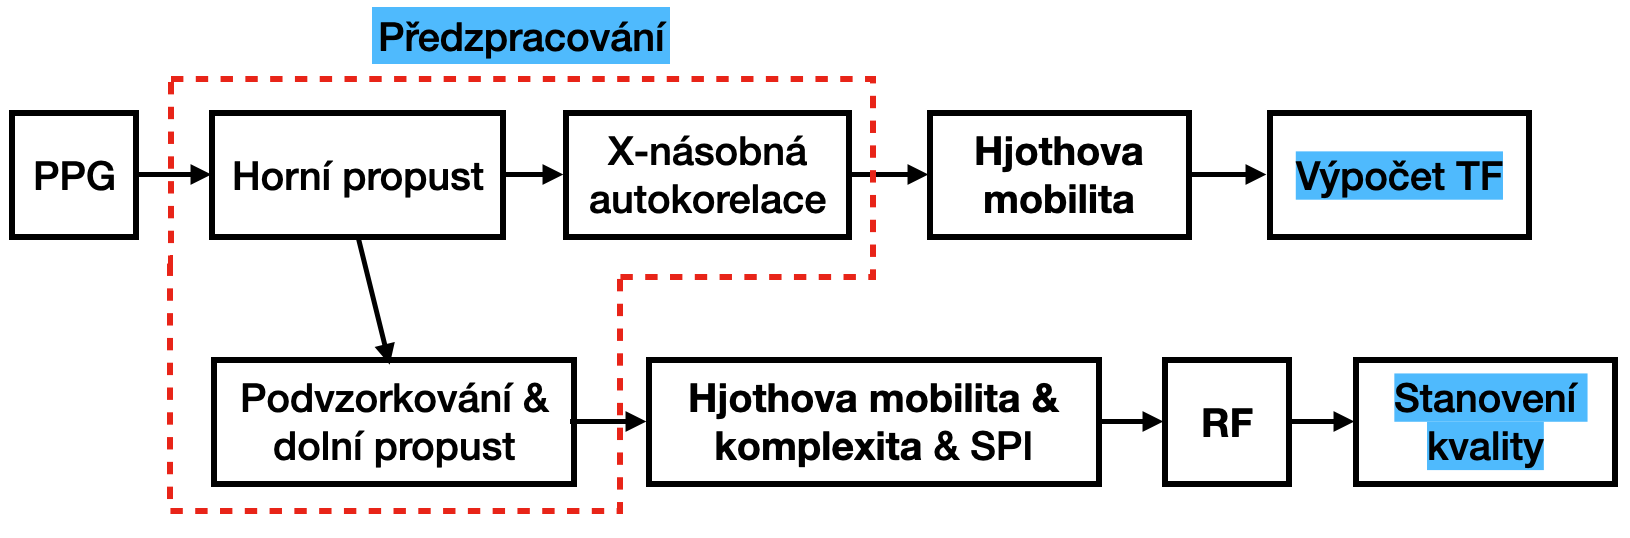
\includegraphics[width=1\textwidth]{./obrazky/hjorth_schema.png} % aktualizovat pro hodnocení kvality?
	\caption[Schéma našeho algorimu, který využívá Hjorthových deskriptorů]{Blokové schéma našeho využití Hjorthových deskriptorů.}
	\label{fig:hjorth_schemata}
\end{figure}

\section{Zpracování signálu}
\label{sec:zpracovani}
% High-pass filtraci pro odstranění DC a respirační složky.
% Jak fungiuje autokorelace (dvakrát) - cílem je zvýraznění periodické složky.
% Grafy autokorelace, původní signál, frekvenční spektrum obou signálů.

\section{Výpočet Hjorthových parametrů}
\label{sec:hjorth_parametery}
% Popis výpočtu Hjorthových parametrů.
% Vysvětlení, co znamenají jednotlivé parametry.
% Které parametry se používají pro výpočet TF.
% Výpočet TF z Hjorthových parametrů (mobility) - vzorec.

